\chapter{Deseño do simulador}
\label{chap:deseño_simulador}

\lettrine{P}{reviamente} a crear calquera programa é necesario un deseño. Durante este capítulo explicaranse as distintas decisións tomadas ao longo do traballo, a súa motivación e alternativas. Ademais, falarase sobre características deste, como a parametrización ou o nivel de funcionamento.

\section{RTL}\label{sec:rtl}
O nivel de simulación é o seguinte paso despois de decidir que arquitectura modelar. Neste caso, decidiuse que o simulador traballe a \acrshort{rtl} debido ao interese en reflexar todas as operacións, a actualización de valores nos rexistros ou non omitir a implementación da conexión dos módulos (unhas das partes máis interesantes neste traballo) ~\cite{rtl_wikipedia}.

Se ben unha alternativa interesante sería \acrshort{tlm}, que é o seguinte nivel de deseño electrónico, a abstracción que proporciona neste caso é demasiado alta para os detalles máis relevantes deste proxecto.  

Tipicamente, para este nivel tan baixo, o habitual é empregar \acrshort{vhdl} ou Verilog. Como se comentou no capítulo \ref{sec:vhdl_verilog} e en \ref{sec:systemc}, SystemC foi elixido por ser máis rápido para simulación, permite traballar a máis nivel e a base do proxecto sobre a que se traballa xa estaba feita cunha linguaxe de alto nivel.

\section{Pipeline de 5 etapas}\label{sec:pipeline_5etapas}
A división do pipeline comeza co nacemento dos primeiros ordenadores segmentados en 1941, aínda que non se popularizaron ata os anos 70 ~\cite{wiki_segmentacion}. A idea é aumentar o rendemento ao permitir que o procesador execute máis dunha instrución por ciclo. Para iso, a versión máis básica é a \acrfull{risc} como se mostra na imaxe \ref{fig:pipeline5etapas}, formada por 5 etapas: Fetch, Decode, Execute, Memory e Write Back.

En Fetch obténse a instrución de memoria. Durante Decode procésase a instrución obtida, analizando que tipo de operación se realizará, cales son os rexistros empregados, se hai algunha dependencia, etc. En Execute realízase a operación determinada, como pode ser un cálculo na \acrfull{alu}. En Memory, se é necesario, escríbese ou léese en memoria. Finalmente, en Write Back actualízanse os rexistros.

Ao deseñar o simulador elixiuse un pipeline de 5 etapas debido á súa sinxeleza. A aproximación realizada foi dividir cada etapa en un módulo do simulador, salvando Decod e Write Back que se uniron por comodidade.

\begin{figure}[hp!]
  \centering
  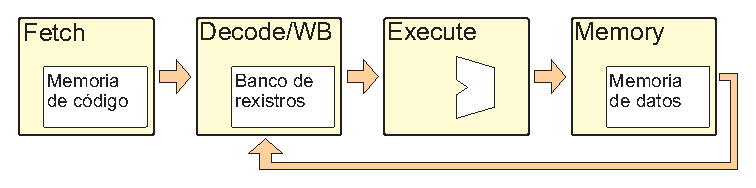
\includegraphics[width=\textwidth]{imaxes/pipeline5etapas.EPS}
  \caption{Figura onde se motra a estrutura do pipeline de 5 etapas.}
  \label{fig:pipeline5etapas}
\end{figure}

\section{Módulos do simulador}\label{sec:modulo_sim}
Os módulos principais, como se comentou no apartado anterior, son cada unha das 5 etapas, fusionando Decod e Write Back. No caso da etapa Execute, simplemente se creou unha \acrshort{alu}, encargada de realizar operacións de suma, resta e outras operacións lóxicas. Ademais, engadíronse varios módulos ao longo do proxecto. Para as operacións de multiplicación e división da extensión M, creouse un novo módulo conectado directamente con Decod, como se pode ver na figura \ref{fig:pipelineMult}. Separar estas funcionalidades permite organizar o traballo, ademais de simplificalo e facerlo máis sinxelo de depurar. Para a extensión F, de forma análoga, existe un compoñente encargado de realizar todas as operacións de punto flotante simple. Estes dous últimos módulos inclúen a posibilidade de parametrizar as súas instrucións, podendo elixir a latencia de determinadas instrucións ou cambiar o funcionamento do módulo (ver \ref{sec:modos_op}).

\begin{figure}[hp!]
  \centering
  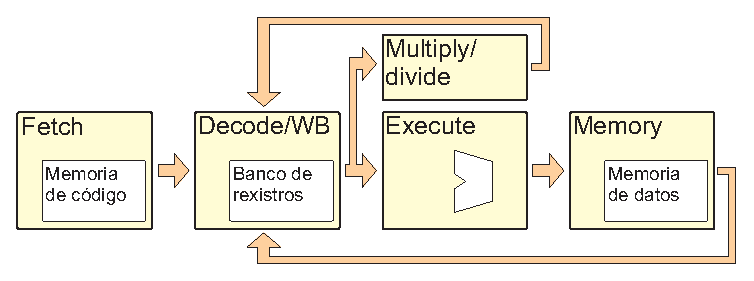
\includegraphics[width=\textwidth]{imaxes/pipelineMult.EPS}
  \caption{Esquema sobre o pipeline do módulo de multiplicación.}
  \label{fig:pipelineMult}
\end{figure}

\section{Modos de operación}\label{sec:modos_op}
Coa fin de mellorar a calidade da simulación, decidíuse engadir no módulo de multiplicación a posibilidade de elixir entre dous modos de funcionamento. O primeiro limita de forma que, se hai unha multiplicación executándose, non se pode realizar ningunha outra operación no módulo. Isto pretende semellarse a un caso real, no que, por limitacións físicas, se empregan os mesmos circuítos para ambas operacións. O segundo modo permite que se executen todas as multiplicacións necesarias, pero só unha división ao mesmo tempo, simulando que existe un circuíto para as divisións e que este só pode realizar unha á vez.


\section{Simulación de latencias}\label{sec:sim_latencias}
Á hora de executar código, existen varios axustes que se poden cambiar para simular distintos comportamentos típicos de RISC-V. Pódese modificar a latencia  das operacións do módulo de multiplicación, as cales son: 
\begin{itemize}
    \item MUL
    \item MULH
    \item MULHU
    \item MULHSU
    \item DIV
    \item DIVU
    \item REM
    \item REMU
    \item FADD.S
    \item FSUB.S
    \item FMUL.S
\end{itemize}
Isto permite unha representación máis realista, xa que por defecto todas as instrucións no simulador teñen unha latencia dun ciclo durante a etapa de Execución. Sen embargo, na realidade, operacións máis complexas como as multiplicacións ou divisións levan varios ciclos.

\section{Sinais de hazard}\label{sec:hazards}
Como sucede en todas as \gls{arquitecturas} segmentadas, a execución de instrucións moitas veces vese limitada por dependencias. Isto é, non se pode continuar co programa porque a seguinte instrución emprega algún rexistro que debe ser actualizado previamente, pero aínda non sucedeu porque algunha instrución anterior non acabou a súa execución. Para evitar esta situación, en moitos casos engádense burbullas, ciclos nos que non se fai ningún traballo para permitir que o resto de instrucións finalicen. O simulador replica este funcionamento, polo que para detectar estas dependencias emprega sinais de \gls{hazards}.

Chámase hazard a calquera perigo que puidese causar un risco \acrfull{raw}, \acrfull{war} ou \acrfull{waw}. Polo que, para evitalo, débese detectar unha dependencia cunha suficiente antelación. A nosa solución neste caso foi empregar sinais nos módulos de punto-flotante, multiplicación e \acrshort{alu} conectados co módulo de decodificación. Se unha dependencia é detectada, o sinal enviará unha alerta ao módulo e este creará burbullas ata que non exista a dependencia.